\chapter{Choosing the Distance between DRPs}
\label{choosingDistance}
In this section we present some considerations on how to choose the 
distance $d$ along the path between two DRs.

\subsection{The Defect} 
\index{Defect}
\index{False Positives}
\index{False Negatives}
\begin{figure}

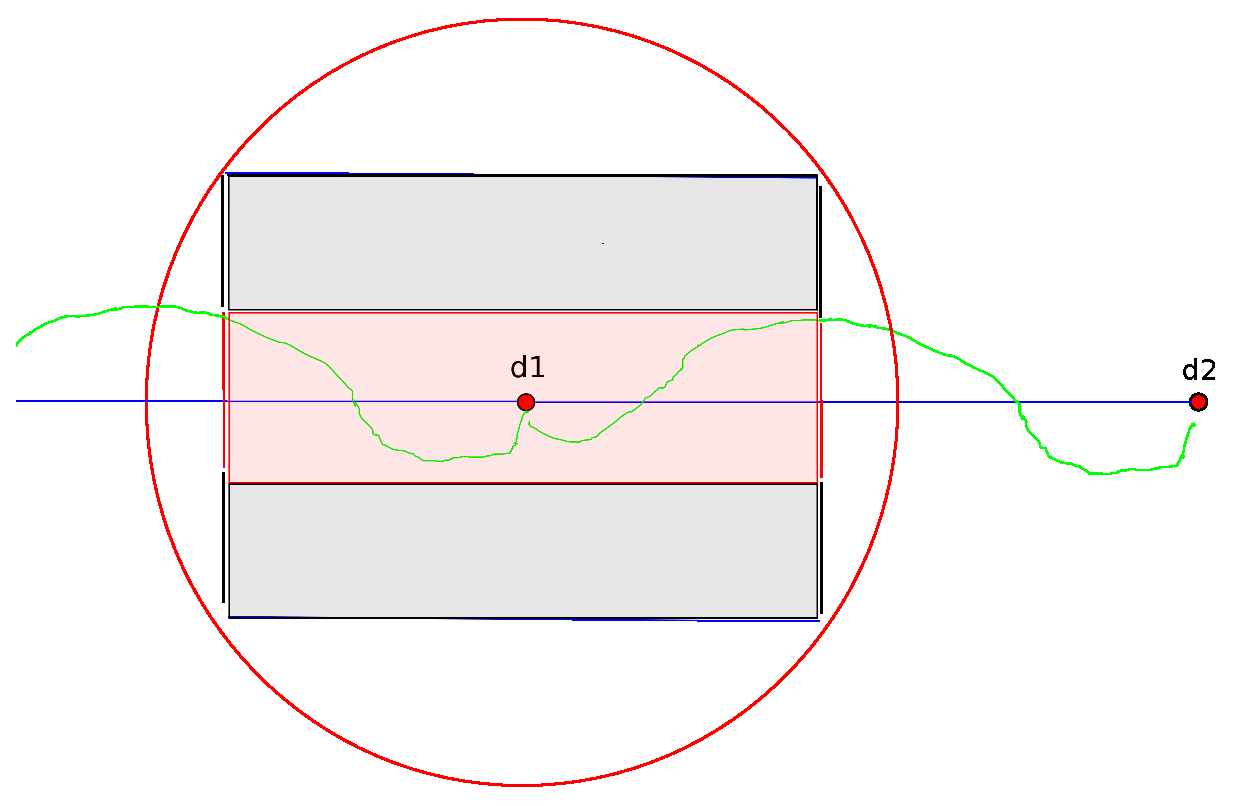
\includegraphics[scale=0.5]{images/04.01.defect.eps}
\caption{Demonstating the \emph{"Defect"}: All points within the \emph{red bar} have 		
         a distance not greater than h from the direct line, while all the points
	inside the gray bars have distance greater than $h$, but less than $h+dist$.
	All points locate inside either grey or red bars can be considered a success,
	while points located inside the circle of radius $t_r$ but outside the 
	bars can be considered  "false positives".
	}
\label{generalDefectFigure}
\end{figure}
\index{False Positives}
\index{False Positives!Ratio between false positives and false negatives}
\index{False Negatives!Ratio between false positives and false negatives} 
A general measure and formula for the defect can be derived from figure \ref{generalDefectFigure}:
All positives are located inside the circle of testradius $t_r$ around $d_1$.
Of these, the \emph{"true positives"} are contained in the rectangle $F$ with height $2*h+2*dist$
and width $\tilde{d}$, where $\tilde{d}$ is the maximum of the direct distance between 
$d_1$ and either its left or right neighbor DR. 
To get a measure for the expected defect, we have to calculate the difference between 
the measure of the circle containing \emph{all positives} and the rectangle containing the \emph{true positives}:

\index{Defect!General Formula}

\begin{equation}
\label{generalDefectFormulaFormally}
	D:=\pi*{t_r}^2-F
\end{equation}

From figure \ref{generalDefectFigure} the identity $F=(\tilde{d}*2(h+dist))$ can be read.
When this is substituted into the definition \ref{generalDefectFormulaFormally},
the definition takes on the form:

\index{Defect!Special Formuula}
\begin{equation}
\label{generalDefectFormula}
        D:=\pi*{t_r}^2-(\tilde{d}*2(h+dist))
\end{equation}

In the rest of this section, we discuss how  the ratio between true positives and false positives 
can be minimized by a sensible choice of the parameter $d$. 

Assuming that interesting points are uniformly distributed in the plane, the
ratio between D and F is a measure for the ratio between all positives and false positives.
This gives:

\index{Defect!Defect Ratio Formula}

\begin{equation}
\label{defectRatioFormula}
        \frac{D}{F}=\frac{\pi*{t_r}^2-(\tilde{d}*2(h+dist))}{(\tilde{d}*2(h+dist))}
\end{equation}


Hoever simple formula \ref{generalDefectFormula} may seem, keep in mind that the formal 
parameters $t_r$ and $\tilde{d}$ may themselves depend on the choice of $d$, while the 
deflection $h$ may vary between 0 and $d$ and depends on geography -- which  is largely out 
of \emph{our} control too.

For this reason, in what follows we discuss the optimal choice of $d$ for some 
special cases only.

\section{Choosing $d$ for a straight Path}

In this section, we discuss the choice of d in case of a straigh path.
For a straight path, we have that the deflection is zero, i.e:
\begin{equation}
 \label{straightDeflection}
  h=0
\end{equation}
and that the direct line between two DRPs is equal to the path between these DRPs, i.e:

\begin{equation}
 \label{straightPath}
  \tilde{d}=d
\end{equation}

Such that the formula for the general defect $D$ \label{generalDefectFormula} 
simplifies to
\begin{equation}
 \label{defectStraightPath}
	D:=\pi*{t_r}^2 -(d*2*dist)
\end{equation}

While $F$ becomes
\begin{equation}
  F:=(d*2*dist)
\end{equation}


Giving the following simplified formula for $\frac{D}{F}$:
\begin{equation}
label{DF_straight_line}
	\frac{D}{F}=\frac{\pi*{t_r}^2 -(d*2*dist)}{d*2*dist} 
\end{equation}

Where the formal parameter $t_r$ might still implicitely contain $d$ !


\subsection{Optimal Choice of d for Straight Line and Testradius $t_{r3}$}

Substituting the $t_{r3}$ as defined in  \label{testradius_tr3},
formula \ref{DF_straight_line} becomes:
\begin{equation}
\label{DF_straight_line_tr3}
\frac{D}{F}=\frac{\pi(\frac{1}{2}d^2+d*dist+dist^2) -(d*2*dist)}{d*2*dist}
\end{equation}

Which becomes minimal for choosing $d$ as:
\begin{equation}
\label{optimal_d_straight_line_tr3}
 d:=(1-dist)+\sqrt{1-2*dist+dist^2-\frac{d*dist^2}{\pi}} 
\end{equation}
















